\addcontentsline{toc}{chapter}{An interesting projection}
\chapter*{An interesting projection}

The end of this project would be to turn it into a scientific game. It should be updated regularly and developed over time. The environments would be more and more sophisticated/realistic as updates are made. Instead of confronting territories with each other, we would confront the intelligence of players on the same territory with identical conditions. Who will best optimize overall harmony ? We would explore all possible realistic dynamics of our world. For example, we could implement the game in a centralized server and leave access to players directly from the internet. Gambling would be accessible to everyone without discrimination, and in most parts of the world. It would be necessary to adapt the calculation performance for the fluidity of the game and to attract players. But it will then be possible to record the results experienced directly in a database. Such registration could even avoid recalculating current environmental assessments, and simply return the recorded results. The more we participate, the more robust the optimizations would be. We would then combine the exploration of environmental solutions, local exploitation and learning by reinforcing our decisions on the management of the world. Of course, a local interest may be preferred in a practical case. It would be more of a local optimization of the world, and the goal would then be to make it global.\\

Could we add additional layers of environment ? A climatological environment, a seismological environment, an ethological environment, and any other scientific environment in the world, through the study of volcanoes, nuclear hazards, clean oceans, etc.\\
 
It would also be an excellent form of education to deepen our understanding of science or develop passions/interests in everyone, as long as it is stimulating. Not to mention that this could encourage many people to orient themselves in computer science, statistics, artificial intelligence, optimization, etc. It would promote a benevolent outlook towards the world. Curious young people who want to learn like the great scientific experts would be satisfied on all sides. We could then rally the population around the humanitarian debate and develop interest in anticipating and optimizing civilization, orienting ourselves in human benevolence and respect for moral principles. Collective intelligence will be used for global harmony. This could even encourage people in the poorest regions to contribute to healthy local data: epidemics, demographics, cartographs, etc. And above all, we could make artificial intelligence accessible to all, by orienting it with a view to global harmony, and not only to a rich elite who could be led to increase entropy.\\

With true transparency and open-mindedness, we could seek to optimize :\\

\begin{itemize}
\item Green energy management.
\item Managing the planet's resources.
\item Humanitarian crisis management.
\item Protection of ecosystems and living beings.
\item Anticipation of natural disasters.
\item Anticipation of demographic changes.
\item Anticipation of climate change.
\item etc.\\
\end{itemize}

Optimal solutions could be found to the seemingly impossible problems of civilization.\\

\texttt{\Large \comfortaa We could revolutionize the world.}

\vspace{1cm}

\begin{center}
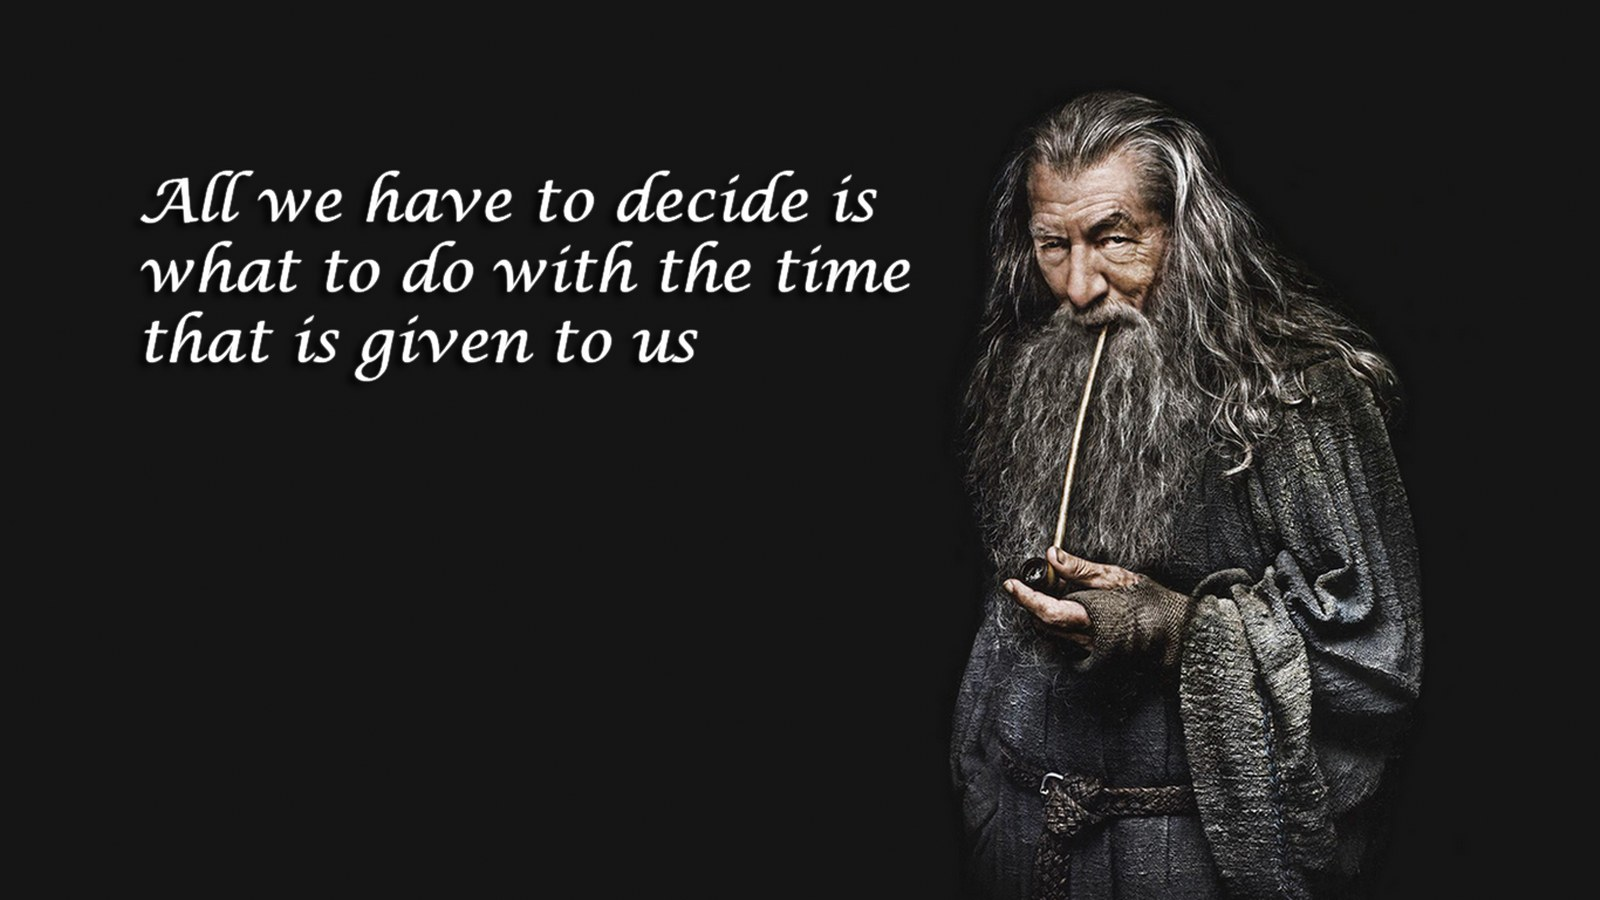
\includegraphics[scale=0.22]{Media/GandalfQuote.jpg}
\end{center}